%% ICML 2026 style (preprint option), anonymous authors. Build: tectonic main.tex
%% 2026-11-16: AndroidControl-only version. Numbers: benchmarks/train/paper_ac_final.py -> paper_numbers.json.
\documentclass{article}

\usepackage[T1]{fontenc}
\usepackage[table]{xcolor}
\usepackage{microtype}
\usepackage{graphicx}
\usepackage{booktabs}
\usepackage{multirow}
\usepackage{array}
\usepackage{xurl}
\usepackage{hyperref}
\newcommand{\theHalgorithm}{\arabic{algorithm}}

\usepackage[preprint]{icml2026}

\usepackage{amsmath}
\usepackage{amssymb}
\usepackage[capitalize,noabbrev]{cleveref}
\newcommand{\BASEAURC}{0.420}
\newcommand{\BASEAUROC}{0.721}
\newcommand{\BASEBOUNDHIGH}{44.2}
\newcommand{\BASEBOUNDLOW}{62.5}
\newcommand{\BASECOVFIFTEEN}{1.1}
\newcommand{\BASECOVTWENTY}{2.5}
\newcommand{\BASEDONEHIGH}{340}
\newcommand{\BASEDONELOW}{231}
\newcommand{\BASEECE}{0.226}
\newcommand{\BASEESRHIGH}{9.4}
\newcommand{\BASEESRLOW}{18.8}
\newcommand{\BASEFIFTEENSPLITS}{2}
\newcommand{\BASEGAP}{22.6}
\newcommand{\BASEGATE}{--}
\newcommand{\BASEHIGH}{40.2}
\newcommand{\BASELOW}{59.8}
\newcommand{\BASEMEANCONF}{62.7}
\newcommand{\BASEPRODAUROC}{0.671}
\newcommand{\BASERISK}{44.2}
\newcommand{\BASERISKFIFTEEN}{21.3}
\newcommand{\BASERISKTWENTY}{19.5}
\newcommand{\BASETENSPLITS}{0}
\newcommand{\BASETWENTYSPLITS}{13}
\newcommand{\BASETYPE}{0.668 / 0.059}
\newcommand{\BASETYPEAUROC}{0.668}
\newcommand{\BASETYPEECE}{0.059}
\newcommand{\BASEVIOLFIFTEEN}{100}
\newcommand{\BASEVIOLTWENTY}{31}
\newcommand{\CURBOX}{73.6}
\newcommand{\CURHARD}{77.0}
\newcommand{\CURLOW}{89.7}
\newcommand{\DIFFCIHIHIGH}{35.5}
\newcommand{\DIFFCIHILOW}{32.1}
\newcommand{\DIFFCILOHIGH}{32.6}
\newcommand{\DIFFCILOLOW}{29.4}
\newcommand{\DIFFHIGH}{34.0}
\newcommand{\DIFFLOW}{30.7}
\newcommand{\ERRARGHIGH}{1{,}081}
\newcommand{\ERRCLICKSCROLLHIGH}{413}
\newcommand{\ERRCLICKTARGETHIGH}{907}
\newcommand{\ERRCLICKWAITHIGH}{247}
\newcommand{\ERRHIGH}{2{,}178}
\newcommand{\ERRTYPEHIGH}{1{,}097}
\newcommand{\OURSAURC}{0.135}
\newcommand{\OURSAUROC}{0.731}
\newcommand{\OURSCIHIHIGH}{75.3}
\newcommand{\OURSCIHILOW}{91.3}
\newcommand{\OURSCILOHIGH}{73.1}
\newcommand{\OURSCILOLOW}{89.7}
\newcommand{\OURSCOVFIFTEEN}{49.7}
\newcommand{\OURSCOVTEN}{10.0}
\newcommand{\OURSCOVTWENTY}{80.5}
\newcommand{\OURSECE}{0.145}
\newcommand{\OURSESRHIGH}{30.6}
\newcommand{\OURSESRLOW}{63.8}
\newcommand{\OURSFIFTEENSPLITS}{200}
\newcommand{\OURSGAP}{14.5}
\newcommand{\OURSGATE}{80.5 / 19.0}
\newcommand{\OURSMEANCONF}{88.7}
\newcommand{\OURSPRODAUROC}{0.749}
\newcommand{\OURSRISK}{13.6}
\newcommand{\OURSRISKFIFTEEN}{13.7}
\newcommand{\OURSRISKTEN}{3.8}
\newcommand{\OURSRISKTWENTY}{19.0}
\newcommand{\OURSTENSPLITS}{194}
\newcommand{\OURSTWENTYSPLITS}{200}
\newcommand{\OURSTYPE}{0.818 / 0.019}
\newcommand{\OURSTYPEAUROC}{0.818}
\newcommand{\OURSTYPEECE}{0.019}
\newcommand{\OURSVIOLFIFTEEN}{14}
\newcommand{\OURSVIOLTEN}{5}
\newcommand{\OURSVIOLTWENTY}{19}
\newcommand{\PAIREDEXP}{100}
\newcommand{\SEEDMEANHIGH}{74.0}
\newcommand{\SEEDMEANLOW}{90.7}
\newcommand{\SEEDN}{3}
\newcommand{\SEEDRANGEHIGH}{0.8}
\newcommand{\SEEDRANGELOW}{0.4}
\newcommand{\SEEDSDHIGH}{0.4}
\newcommand{\SEEDSDLOW}{0.2}


\definecolor{oursbg}{HTML}{E3ECF8}
\newcolumntype{L}[1]{>{\raggedright\arraybackslash}p{#1}}
\newcommand{\ours}{DMA-2B}
\newcommand{\base}{d1-2B}
\makeatletter\newcommand{\inputrows}[1]{\@@input #1 }\makeatother

\icmltitlerunning{Single-Pass Action Selection for Mobile GUI Control}

\begin{document}

\twocolumn[
  \icmltitle{Single-Pass Action Selection for Mobile GUI Control:\\A 2B Decision Model on AndroidControl}

  \begin{icmlauthorlist}
    \icmlauthor{Anonymous Author(s)}{anon}
  \end{icmlauthorlist}
  \icmlaffiliation{anon}{Anonymous institution}
  \icmlcorrespondingauthor{Anonymous Author(s)}{anonymous@example.com}
  \icmlkeywords{GUI agents, decision models, calibration, selective prediction, AndroidControl}
  \vskip 0.3in
]

\printAffiliationsAndNotice{}

\begin{abstract}
Most mobile GUI agents are vision-language models that write a reasoning trace and an action string at every
step. A \emph{decision model} works differently: it reads the screenshot and the list of screen elements once and
returns a probability for each possible answer in a single forward pass, without generating any text. We fine-tune the 2B decision model
\base{} on the AndroidControl training split and call the result \ours{}. With the InfiGUI-R1 evaluation code,
\ours{} reaches a step success rate of 90.5\% on AndroidControl-Low and 74.2\% on AndroidControl-High in
AndroidControl's own action space, up from \BASELOW\% and \BASEHIGH\% for the base model; retraining with two other
seeds gives the same result within one point. On AndroidControl-High this is the best reported result for a 2B model
and above several generative agents of 7B to 8B parameters. On AndroidControl-Curated it reaches \CURLOW\% (Easy) and \CURHARD\% (Hard), above every model
the benchmark's authors report. Because every answer comes with a probability, the agent can decide when to act and
when to ask: with a threshold chosen on held-out episodes for a 20\% risk target, it acts on \OURSCOVTWENTY\% of the
steps with a mean error rate of \OURSRISKTWENTY\%.
\end{abstract}

%% ==================================================================
\section{Introduction}
\label{sec:intro}

Most mobile GUI agents are generative. At each step a vision-language model (VLM) reads a screenshot, writes
a thought, and emits the action as text, which the harness then parses and executes
\citep{uitars2025,mobileagentv3,mobilerl2025}. On a phone this has three costs. The action is a string, so a
malformed output becomes a runtime error. Decoding is sequential, so each step takes longer as the reasoning
grows. And the agent gives no probability for its action, so the software around it cannot tell when to act,
when to ask the user and when to stop.

A decision model avoids all three \citep{typesafe2026,liquidd12026}. It receives a state and a set of typed
questions and returns, for each question, a probability over a closed set of answers in one forward pass. The
output always fits the schema, the cost is one forward pass, and every answer has a probability. This paper
measures how well such a model selects phone actions on a standard benchmark, AndroidControl
\citep{androidcontrol2024}, and how useful its probabilities are. Our contributions are:
\begin{enumerate}
  \item A single-pass decision interface for mobile GUI control built on an open decision model
        (\cref{sec:method}): the action, the target element, the scroll direction, the app and any text to type
        all come from one forward pass.
  \item \ours{}, a 2B decision model fine-tuned on the full AndroidControl training split, with 90.5\% (Low) and
        74.2\% (High) step success, against \BASELOW\% and \BASEHIGH\% for the base model, and the same result
        across training seeds (\cref{sec:results}).
  \item A study of the action probability as a control signal: how well it ranks errors, and which error rate a
        threshold chosen on held-out episodes achieves (\cref{sec:confidence}).
\end{enumerate}

%% ==================================================================
\section{Related Work}
\label{sec:related}

\paragraph{Mobile GUI agents.}
AndroidControl \citep{androidcontrol2024} scores individual steps of human demonstrations in two settings: with
the step instruction (Low) and with the goal only (High). Recent agents are VLMs trained with supervised
fine-tuning on GUI trajectories \citep{osatlas,aguvis,uitars2025} and, increasingly, with reinforcement learning
from rule-based or environment rewards \citep{uir1,guir1,infiguir1,uigenie,mobilerl2025}. All of them generate
text, and several generate an explicit reasoning trace before the action.

\paragraph{Decision models.}
TypeSafe's Jev and LiquidAI's d1 family answer typed questions (choice, yes/no, score, span, box) in one pass and
return probabilities rather than text \citep{typesafe2026,liquidd12026}. Two recent mobile agents also select
actions without decoding text: Jev-Mobile \citep{jevmobile2026} lets a VLM planner set a sub-goal and a Jev decision
model pick the actions from the accessibility tree, and GUI-JEPA \citep{guijepa2026} scores candidate actions in the
latent space of a screenshot encoder in one batched pass. We build on the open d1-2B model and train it to choose
every part of the action, including when an instruction is done.

\paragraph{Calibration and selective prediction.}
A classifier is calibrated when its confidence matches its accuracy \citep{guo2017calibration}. Selective
prediction lets a model abstain where its confidence is low and trades coverage for risk
\citep{geifman2017selective}. Learn-then-Test \citep{angelopoulos2021ltt} and conformal risk control
\citep{angelopoulos2024crc} turn a score into a threshold with a finite-sample guarantee on the risk of the
accepted decisions. CORA \citep{cora2026} applies conformal risk control to mobile GUI automation with a separate
guardian model; we apply the same tools to the probability that the acting model itself produces.

%% ==================================================================
\section{Method}
\label{sec:method}

\subsection{Problem formulation}
At step $t$ the agent observes a screenshot $x_t$ and the accessibility tree of the screen, and knows the goal
$g$, optionally the step instruction $u_t$, and its previous actions $h_{<t}$. A deterministic renderer turns
$(g, u_t, h_{<t}, \text{tree})$ into a text state $z_t$ that lists the goal, the instruction, the current app,
the previous actions with their observed effects, and the visible elements
$\mathcal{E}_t = \{e_1,\dots,e_{n_t}\}$ with label, type, state and position. The model receives
$s_t = (x_t, z_t)$ and a fixed set of typed questions, and returns in one forward pass
\begin{equation}
  p(a \mid s_t),\; p(e \mid s_t),\; p(d \mid s_t),\; p(m \mid s_t),\; p(\sigma \mid s_t),
\end{equation}
where $a$ is the action type, $e \in \mathcal{E}_t$ the target element, $d$ the scroll direction, $m$ the app to
open, chosen from a list of installed apps, and $\sigma$ a span of $z_t$ that is copied as the text to type. The
executed action is assembled from the arg-max answers. Because spans are copied from the text state, the model
cannot produce text that appears only in the pixels.

\subsection{Model and training data}
The decision model is \base{} \citep{liquidd12026}, a 1.92B-parameter vision-language decision model whose readout
heads project the backbone state onto the token groups of each question's options. We fine-tune all parameters,
including the vision encoder, except the tied input embedding and output head, with a cross-entropy loss on every
question that the gold action defines. Each previous action in the state is written with the element it acted on and
its effect, ``screen changed'' or ``no change'', which is computed by comparing the element lists before and after
the action (system UI and the keyboard are ignored). The screenshot is resized to 720 pixels wide.

The training data are built from the complete AndroidControl training split, rebuilt from the original release:
13{,}594 episodes and 88{,}308 steps, with every test episode excluded. A fixed share of the episodes (34\%) is
shown with the goal only, as in the High setting. In the remaining episodes the step instructions are grouped into
\emph{local goals} of one to four consecutive instructions, and every step shows the instructions of its local
goal; after the last step of each local goal, the next screen is added with the answer ``done'', so the model also
learns when an instruction has been carried out. Steps that continue an instruction from the previous step
(AndroidControl repeats an instruction over several steps, for example for repeated scrolls or a wait after a
click) are repeated three times. A row is one training example (one screen with its questions and answers); the
training set has 116{,}139 rows. We train for 7{,}000 optimizer steps with batches of 16 rows, using 8-bit AdamW
without weight decay, learning rate $10^{-5}$ with 30 warm-up steps and a cosine decay, gradient clipping at 1.0 and
bf16 weights, which takes about 16 hours on one RTX 4090. The released model is seed 0; \cref{sec:seeds} repeats the
training with other seeds.

\subsection{Scoring}
The AndroidControl action space has no ``done'' action, and the test split contains no step whose correct action
is ``done''. We therefore score \ours{} in AndroidControl's own action space: the ``done'' option is removed at
inference and the best remaining action of the same forward pass is taken. \Cref{sec:ablations} reports what
happens when it is not removed. The base model receives the same input and questions and is reported with its full action space, in which it
answers ``done'' on \BASEDONELOW{} (Low) and \BASEDONEHIGH{} (High) of the 8{,}444 steps; even if each of these
answers were replaced by a correct action, it would reach at most \BASEBOUNDLOW\% and \BASEBOUNDHIGH\%.

\subsection{Confidence and escalation}
\label{sec:gate}
We use the probability of the selected action, $c(s_t) = p(\hat a \mid s_t)$, as the step confidence. An
escalation gate acts if $c(s_t) \geq \tau$ and asks otherwise. For $n$ scored steps with correctness
$y_i \in \{0,1\}$, coverage and selective risk are
\begin{align}
  \mathrm{cov}(\tau) &= \frac{1}{n}\sum_{i=1}^{n} \mathbf{1}[c_i \geq \tau], \\
  R(\tau) &= \frac{\sum_{i} \mathbf{1}[c_i \geq \tau]\,(1-y_i)}{\sum_{i} \mathbf{1}[c_i \geq \tau]}.
\end{align}
To choose $\tau$ for a target risk $\delta$ we follow Learn-then-Test with fixed-sequence testing
\citep{angelopoulos2021ltt}: on a calibration set we sort the steps by confidence, accept them one at a time from the
most confident, and stop before the first accepted set (of at least 30 steps) whose one-sided Clopper--Pearson upper
bound on the error rate at level $\alpha = 0.05$ exceeds $\delta$. With probability at least $1-\alpha$ over the
calibration set, the error rate of the chosen gate on new steps from the same distribution is then at most $\delta$.

%% ==================================================================
\section{Experimental Setup}
\label{sec:setup}

The AndroidControl test split has 8{,}444 steps in 1{,}543 episodes \citep{androidcontrol2024}. In the Low setting
the model sees the step instruction; in the High setting it sees only the goal. In both settings the history is
the demonstrator's, so every step is evaluated from the correct prefix. We score with the evaluation code of
InfiGUI-R1 \citep{infiguir1} without modification and report \emph{Type}, the action-type accuracy;
\emph{Grounding}, the share of click and long-press steps with the correct type whose predicted point falls inside
the target element; \emph{SR}, the step success rate; and the \emph{episode success rate} (ESR), the share of
episodes in which every step is correct. Decoding is a single deterministic forward pass. We compare against the
untrained base model and against the results reported for other models. Intervals are 95\% bootstrap intervals over
episodes (2{,}000 resamples), since the steps of one episode are not independent.

%% ==================================================================
\section{Results}
\label{sec:results}

\begin{table}[!t]
\centering
\caption{Step success rate (\%) on the AndroidControl test set (8{,}444 steps). Rows of other models are the
values reported in the papers listed in \cref{sec:ac}; prompts, action spaces and scorers differ between
sources, so the comparison is approximate. Text: the model generates text. $^{\dagger}$500 sampled steps.
$^{\ddagger}$7{,}708 test steps.
``--'': not reported. Bold: best.}
\label{tab:ac}
\small
\setlength{\tabcolsep}{4.5pt}
\begin{tabular}{@{}l r c r r@{}}
\toprule
Model & Size & Text & Low & High \\
\midrule
\inputrows{tables/tab_ac_rows.tex}
\bottomrule
\end{tabular}
\end{table}

\begin{table*}[t]
\centering
\caption{Base model and \ours{} on the AndroidControl test set, InfiGUI-R1 scorer. \ours{} is scored in
AndroidControl's action space, the base model with its full action space (\cref{sec:method}). ESR: episodes in
which every step is correct (1{,}543 episodes).}
\label{tab:ours}
\small
\setlength{\tabcolsep}{6pt}
\begin{tabular}{@{}l cccc cccc@{}}
\toprule
& \multicolumn{4}{c}{AndroidControl-Low} & \multicolumn{4}{c}{AndroidControl-High} \\
\cmidrule(lr){2-5}\cmidrule(l){6-9}
Model & Type & Grounding & SR & ESR & Type & Grounding & SR & ESR \\
\midrule
\inputrows{tables/tab_ours_rows.tex}
\bottomrule
\end{tabular}
\end{table*}

\subsection{AndroidControl}
\label{sec:ac}
\Cref{tab:ours} compares \ours{} with the base model it starts from. Fine-tuning raises step success from
\BASELOW\% to 90.5\% (95\% interval \OURSCILOLOW--\OURSCIHILOW) on AndroidControl-Low and from \BASEHIGH\% to
74.2\% (\OURSCILOHIGH--\OURSCIHIHIGH) on AndroidControl-High. The paired gains are \DIFFLOW{} points
(\DIFFCILOLOW--\DIFFCIHILOW) and \DIFFHIGH{} points (\DIFFCILOHIGH--\DIFFCIHIHIGH). The ``done'' option does not
explain this gap: the base model answers ``done'' on at most \BASEDONEHIGH{} of the 8{,}444 steps, and even if all
these answers were correct it would stay below \BASEBOUNDLOW\% and \BASEBOUNDHIGH\%.

\Cref{tab:ac} places \ours{} among published models. The values are those reported by InfiGUI-R1
\citep{infiguir1} (GPT-4o \citep{gpt4o}, OS-Atlas-4B \citep{osatlas}, Aguvis \citep{aguvis}, UI-TARS-2B
\citep{uitars2025}, InfiGUI-R1-3B), by GUI-R1 under its shared zero-shot prompt \citep{guir1} (Qwen2.5-VL-3B and
7B, UI-R1-3B \citep{uir1}, GUI-R1), by MobileRL \citep{mobilerl2025} (UI-TARS-7B and 72B,
MobileRL), and by each model's own paper for UI-Genie, Qwen2.5-VL-72B \citep{qwen25vl}, MAI-UI \citep{maiui2025}, OS-Atlas-7B
\citep{osatlas}, AgentCPM-GUI \citep{agentcpmgui2025}, GUI-Owl \citep{mobileagentv3}, UI-Venus-Navi
\citep{uivenus2025}, GUI-SAGE \citep{guisage2026}, UI-Genie \citep{uigenie} and OmegaUse \citep{omegause2026}.
Aguvis is scored on 500 sampled steps and OS-Atlas on 7{,}708 steps rather than the full test split. The inputs also differ: \ours{} reads the accessibility element list
and chooses an element, while most of the other models predict a point on the screenshot.

On AndroidControl-High, \ours{} (74.2\%) is the best reported 2B model (UI-TARS-2B 68.9\%, MAI-UI-2B 67.3\%). It is
above AgentCPM-GUI-8B (69.2\%), MAI-UI-8B (69.1\%), OS-Atlas-7B (71.2\%), UI-TARS-7B (72.5\%) and GUI-Owl-7B
(72.8\%), and level with MobileRL-9B (73.9\%) and UI-Genie-7B (74.2\%). Three models of 3B to 7B are higher,
GUI-SAGE-3B (75.4\%), UI-Venus-Navi-7B (76.1\%) and GUI-SAGE-7B (76.8\%), as are six of the eight models of 30B or
more, up to 79.1\% (OmegaUse, a 30B mixture-of-experts model). On AndroidControl-Low, \ours{} (90.5\%) is above
UI-TARS-2B (89.3\%) and AgentCPM-GUI-8B (90.2\%), level with UI-TARS-7B (90.8\%), and 0.8 to 4.3 points below eleven
models of 3B to 72B, the highest being UI-Genie-72B (94.8\%). Every other model in
the table generates text, and several generate a reasoning trace before each action; \ours{} answers every step in
one forward pass.

\subsection{AndroidControl-Curated}
\label{sec:curated}
AndroidControl-Curated \citep{accurated2025} re-scores the same test steps with box-based grounding (the centre of the
prediction must fall inside the target element) and corrects the high-level split; in the released files, 527 tasks
are rewritten, 573 steps accept alternative valid actions and 86 labels are fixed. Its Easy split (8{,}377 steps) corresponds to AndroidControl-Low and its Hard split (8{,}377 steps) to
AndroidControl-High; Hard (Box) is the Hard split with the box metric but the original tasks and labels (8{,}435
steps). We match every
Curated row to its AndroidControl test step through the episode and step in its image path, reuse the predictions of
\cref{sec:ac}, re-run \ours{} only on the 527 rewritten tasks, and score with the authors' rules, which we
re-implemented (the released code states no license). A row-by-row comparison with the authors' own scoring
functions, run on all rows of the three splits, gives the same verdict on every row (0 mismatches). \Cref{tab:curated} lists the step success rates; the other rows
are reported by \citet{accurated2025}. \ours{} has the highest value in all
three columns. The inputs differ: the reported models read the screenshot and a written history of the previous step
instructions, while \ours{} also reads the accessibility element list and the previous actions of the demonstration
with their effects.

\begin{table}[!t]
\centering
\caption{Step success rate (\%) on AndroidControl-Curated. Other rows as reported by the benchmark's authors.
``--'': not reported.}
\label{tab:curated}
\small
\setlength{\tabcolsep}{4pt}
\begin{tabular}{@{}l r r r r@{}}
\toprule
Model & Size & Easy & Hard (Box) & Hard \\
\midrule
UI-R1-3B & 3B & 58.9 & -- & 43.6 \\
GUI-R1-3B & 3B & 67.1 & 49.4 & 54.4 \\
GUI-R1-7B & 7B & 72.7 & 53.2 & 57.5 \\
InfiGUI-R1-3B & 3B & 87.2 & 67.6 & 70.7 \\
Qwen3-VL-30B & 30B & 70.5 & -- & 70.0 \\
Qwen3-VL-235B & 235B & 74.5 & 71.7 & 76.5 \\
Magma-R1 & 3B & 88.0 & 69.1 & 75.3 \\
\midrule
\rowcolor{oursbg}\textbf{\ours{}} & 2B & \textbf{\CURLOW} & \textbf{\CURBOX} & \textbf{\CURHARD} \\
\bottomrule
\end{tabular}
\end{table}

\subsection{Training seeds}
\label{sec:seeds}
\begin{table}[!t]
\centering
\caption{\ours{} trained with different seeds (same data, recipe and checkpoint step), AndroidControl step success
rate (\%) and episode success rate on High (\%).}
\label{tab:seeds}
\small
\setlength{\tabcolsep}{5pt}
\begin{tabular}{@{}l r r r@{}}
\toprule
Training run & Low & High & ESR (High) \\
\midrule
\inputrows{tables/tab_seeds_rows.tex}
\bottomrule
\end{tabular}
\end{table}
We repeated the whole training with two other seeds; the seed changes the order of the training data. \Cref{tab:seeds}
shows that the results agree: \SEEDMEANLOW{} $\pm$ \SEEDSDLOW\% on Low and \SEEDMEANHIGH{} $\pm$ \SEEDSDHIGH\% on High
over \SEEDN{} runs; the step success rates of the runs lie within \SEEDRANGEHIGH{} points of each other. The released
model is therefore a typical result of the recipe, not a lucky run. All other results are for the released model.

\subsection{Latency}
\label{sec:latency}
One decision is one forward pass of the 1.92B model and generates no tokens. We served the
released model over HTTP on one RTX 4090 (24\,GB) and sent 500 AndroidControl-High test steps one at a time (median 55
elements per screen). The forward pass took 123\,ms at the median and 144\,ms at the 95th percentile, and the whole request, timed by the
client on the same host, 133\,ms and 155\,ms. The time barely depends on the length of the element list: 119\,ms below
50 elements and 129\,ms at 150 or more.

%% ==================================================================
\section{Confidence as a Control Signal}
\label{sec:confidence}

\begin{table}[t]
\centering
\caption{Step confidence $c = p(\hat a\mid s)$ on AndroidControl-High (8{,}444 steps). Risk@50: error rate on the
50\% most confident steps. ECE: 15 equal-width bins. Gate: a threshold chosen on half of the episodes for a target risk of 20\%, applied to
the other half (mean over 200 random splits); ``--'': a threshold exists in fewer than half of the splits.}
\label{tab:calib}
\small
\setlength{\tabcolsep}{5pt}
\begin{tabular}{@{}l c c@{}}
\toprule
& \base{} (base) & \ours{} \\
\midrule
SR (\%)                       & \BASEHIGH & 74.2 \\
Mean confidence (\%)          & \BASEMEANCONF & \OURSMEANCONF \\
ECE $\downarrow$              & \BASEECE & \OURSECE \\
AUROC $\uparrow$              & \BASEAUROC & \OURSAUROC \\
Risk@50 (\%) $\downarrow$     & \BASERISK & \OURSRISK \\
AURC $\downarrow$             & \BASEAURC & \OURSAURC \\
Type: AUROC / ECE             & \BASETYPE & \OURSTYPE \\
\midrule
Gate $\delta{=}20\%$: cov. / risk (\%) & \BASEGATE & \OURSGATE \\
\bottomrule
\end{tabular}
\end{table}

\begin{figure}[t]
  \centering
  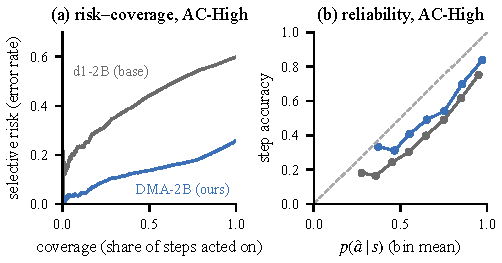
\includegraphics[width=\columnwidth]{figures/fig_calibration.pdf}
  \caption{AndroidControl-High, base model and \ours{}. (a) Error rate among the steps the gate accepts, as the
  threshold is lowered. (b) Step accuracy against confidence in ten equal-width bins (bins with fewer than 20 steps
  omitted); the dashed line is perfect calibration.}
  \label{fig:calibration}
\end{figure}

\Cref{tab:calib} and \cref{fig:calibration} compare the step confidence of the base model and of \ours{} on
AndroidControl-High. Fine-tuning lowers the error rate on the half of the steps the model is most confident about
from \BASERISK\% to \OURSRISK\%, and the area under the risk--coverage curve from \BASEAURC{} to \OURSAURC{}. The
ranking of correct above incorrect steps improves only slightly (AUROC \BASEAUROC{} to \OURSAUROC{}; \OURSPRODAUROC{}
when the action probability is multiplied by the element probability), and both models are over-confident: mean
confidence exceeds accuracy by \BASEGAP{} and \OURSGAP{} points. For the action type alone, the probability of
\ours{} is close to calibrated (ECE \OURSTYPEECE) and ranks type errors with AUROC \OURSTYPEAUROC.

To turn the probability into a gate, we split the test episodes into two halves 200 times, choose $\tau$ on one
half with the procedure of \cref{sec:gate}, and apply it to the other. For a target risk $\delta = 20\%$ a threshold
exists in every split, and the gate acts on \OURSCOVTWENTY\% of the held-out steps with a mean error rate of
\OURSRISKTWENTY\%. For $\delta = 15\%$ it acts on \OURSCOVFIFTEEN\% of the steps (error rate \OURSRISKFIFTEEN\%),
and for $\delta = 10\%$ on \OURSCOVTEN\% (error rate \OURSRISKTEN\%; a threshold exists in \OURSTENSPLITS{} of 200
splits). For the base model a threshold for $\delta = 20\%$ exists in only \BASETWENTYSPLITS{} of 200 splits. The
guarantee holds with probability $1-\alpha$ over the calibration half and concerns new steps; on a finite held-out
half the realised error rate still exceeds $\delta$ in some splits (\OURSVIOLTWENTY\% of them for $\delta = 20\%$).

%% ==================================================================
\section{Episodes and Errors}
\label{sec:episodes}
The AndroidControl scorer feeds the demonstrator's history at every step and never checks the goal, so errors do
not compound. \Cref{fig:episode} shows the episode success rate on AndroidControl-High by episode length.
\ours{} gets every step of an episode right in \OURSESRHIGH\% of the episodes on High and \OURSESRLOW\% on Low,
against \BASEESRHIGH\% and \BASEESRLOW\% for the base model. On High the share falls from 65.5\% for one-step
episodes to 27.7\% for five-step episodes and 5.3\% for episodes of ten steps or more (base model: 48.3\%, 3.9\% and
0\%). Longer episodes give a single mistake more chances to occur.

The \ERRHIGH{} wrong steps on AndroidControl-High split evenly. In \ERRTYPEHIGH{} the action type is wrong; the most
common confusions are click against scroll (\ERRCLICKSCROLLHIGH{} steps) and click against wait
(\ERRCLICKWAITHIGH{}), where the demonstrator waits for a screen that is still loading. In the other \ERRARGHIGH{} the
type is right but the argument is wrong, and \ERRCLICKTARGETHIGH{} of these are clicks on the wrong element.

\begin{figure}[t]
  \centering
  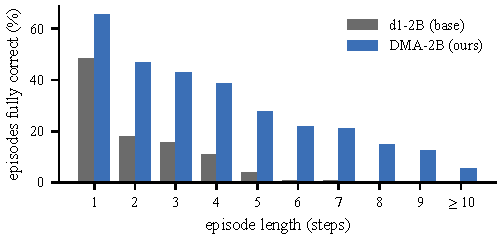
\includegraphics[width=\columnwidth]{figures/fig_episode.pdf}
  \caption{AndroidControl-High: share of episodes in which every step is correct, by episode length (1{,}543
  episodes; 65 to 256 per length).}
  \label{fig:episode}
\end{figure}

%% ==================================================================
\section{Ablations}
\label{sec:ablations}

\begin{table}[t]
\centering
\caption{Ablations, AndroidControl step success rate (\%), InfiGUI-R1 scorer. Steps: optimizer steps. Averaged: weight
average of the two models; repeats: the repeated continuation steps of \cref{sec:method}. Validation: correct steps out
of 690 action steps of the AndroidControl validation split in the Low format.}
\label{tab:abl}
\small
\setlength{\tabcolsep}{4pt}
\begin{tabular}{@{}L{5.7cm} r r@{}}
\toprule
Variant & Low & High \\
\midrule
\rowcolor{oursbg}\ours{} & 90.5 & 74.2 \\
Earlier recipe (40k rows, 2{,}482 steps) & 89.3 & 69.7 \\
``Done'' kept at test time & 86.8 & 74.2 \\
\midrule
& \multicolumn{2}{r}{Validation} \\
\ours{} & \multicolumn{2}{r}{601/690} \\
Averaged with a model without repeats & \multicolumn{2}{r}{606/690} \\
Averaged with the earlier-recipe model & \multicolumn{2}{r}{601/690} \\
\bottomrule
\end{tabular}
\end{table}

\Cref{tab:abl} lists the variants we measured. Our earlier recipe, which trained on a curated 40k-row subset for
2{,}482 optimizer steps without local goals, is 1.2 points lower on Low and 4.5 points lower on High. Leaving the
``done'' option in the action space costs 3.7 points on Low: the model answers ``done'' on 449 of the 8{,}444 steps
where the demonstrator still acts, 359 of them one step early. In 222 of these, AndroidControl keeps the same
instruction for one more step, typically a wait after a click while the next screen loads. It costs nothing on High,
where the model never answers ``done''. Averaging the weights with a model trained without repeated continuation
steps, or with the earlier-recipe model, changes validation accuracy by at most 5 of 690 steps, so we keep the single
model.

%% ==================================================================
\section{Limitations}
The rows of other models come from their papers, which use their own prompts, inputs, action spaces and scorers, so
small differences between rows are approximate; \ours{} needs the accessibility element list of the screen. AndroidControl scores each step from the demonstrator's history; it
measures step accuracy, not task completion. We score in AndroidControl's action space, which has no ``done''
action (\cref{sec:ablations}). The gate of \cref{sec:confidence} assumes that calibration and test steps come from
the same distribution.

\section{Conclusion}
A 2B decision model that answers typed questions in one forward pass, with no generated tokens, reaches 90.5\% and
74.2\% step success on AndroidControl-Low and High, up from \BASELOW\% and \BASEHIGH\% for its base model, and the result
holds across training seeds. On High it is the best reported 2B model and above several generative agents of 7B to 8B
parameters. With its action probability as a gate it acts on \OURSCOVTWENTY\% of the steps at a mean error
rate of \OURSRISKTWENTY\%, which gives an agent a simple rule for when to ask. Half of the remaining errors on High are
in the action type and most of the rest are clicks on the wrong element, so the next gains lie in choosing the
element and in telling when a screen is still loading.

\section*{Impact Statement}
This work aims to make phone agents faster and to let them ask a person before acting when they are unsure. An agent
that acts on a phone can send messages, change settings or make purchases on a user's behalf; the confidence gate
reduces, but does not remove, the risk of wrong actions, and such agents should ask before irreversible steps.

\bibliography{refs}
\bibliographystyle{icml2026}

\end{document}
